\question
Una barra metálica de \qty{100}{\centi\metre} de longitud tiene sus
extremos $x=0$, $x=100$ mantenidos a \qty{0}{\degreeCelsius}.
Inicialmente, la mitad de la barra está a \qty{60}{\degreeCelsius};
mientras que la otra mitad a \qty{40}{\degreeCelsius}.
Asumiendo un coeficiente de difusividad de \num{0.16} unidades c.g.s
y un entorno aislado.
\begin{figure}[ht!]
	\centering
	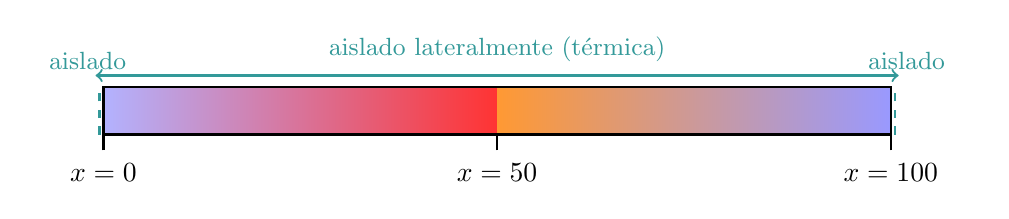
\begin{tikzpicture}
		\shade[left color=blue!30, right color=red!80] (0, 0) rectangle (5, 0.6);
		\shade[left color=orange!80, right color=blue!40] (5, 0) rectangle (10, 0.6);
		\draw[thick, black] (0, 0) rectangle (10, 0.6);
		\draw[thick, dashed, color=teal!80] (-0.05, 0) -- (-0.05, 0.6);
		\draw[thick, dashed, color=teal!80] (10.05, 0) -- (10.05, 0.6);
		\draw[thick] (0, -0.2) -- (0, 0);
		\draw[thick] (5, -0.2) -- (5, 0);
		\draw[thick] (10, -0.2) -- (10, 0);
		\node[below=0.25cm] at (0, 0) {$x=\qty{0}{\centi\metre}$};
		\node[below=0.25cm] at (5, 0) {$x=\qty{50}{\centi\metre}$};
		\node[below=0.25cm] at (10, 0) {$x=\qty{100}{\centi\metre}$};
		\node[above=0.15cm, font=\small, color=white] at (2.5, 0.6) {$T_{0}\left(x\right)=\qty{60}{\degreeCelsius}$};
		\node[above=0.15cm, font=\small, color=white] at (7.5, 0.6) {$T_{0}\left(x\right)=\qty{40}{\degreeCelsius}$};
		\node[above=0.2cm, font=\small, color=white, font=\bfseries] at (0, 0.4) {$T\left(0,t\right)=\qty{0}{\degreeCelsius}$};
		\node[above=0.2cm, font=\small, color=white, font=\bfseries] at (10, 0.4) {$T\left(100,t\right)=\qty{0}{\degreeCelsius}$};
		\node[above=0.3cm, font=\small, color=teal!80] at (-0.2, 0.4) {aislado};
		\node[above=0.3cm, font=\small, color=teal!80] at (10.2, 0.4) {aislado};
		\draw[thick, <->, color=teal!80] (-0.1, 0.75) -- (10.1, 0.75);
		\node[above=0.05cm, font=\small, color=teal!80] at (5, 0.75) {aislado lateralmente (térmica)};
	\end{tikzpicture}
	\caption{Distribución inicial de temperatura en la barra metálica con condiciones de frontera Dirichlet homogéneas.}
\end{figure}

\begin{parts}
	\part\label{1a}

	Describa la ecuación diferencial correspondiente, así como las
	condiciones iniciales y de frontera.

	\part

	No resuelva, solo comente los pasos a tener en cuenta para resolver
	el problema en el ítem~(\ref{1a}).
\end{parts}

\begin{solutionordottedlines}
	El fenómeno físico descrito es un problema de
	\emph{conducción de calor unidimensional en régimen transitorio} en
	un dominio $\Omega=\left[0,L\right]$ donde
	$L=\qty{100}{\centi\metre}$.

	\begin{parts}
		\part

		\begin{equation*}
			\diffp{T}{t}=
			\alpha
			\diffp[2]{T}{x}
			\text{ en }\Omega\times
			\left(0,\infty\right).
		\end{equation*}
		donde
		\begin{itemize}
			\item

			      $T\left(x,t\right)\in\mathbb{R}$ es la temperatura en la
			      posición $x$ al tiempo $t$.

			\item

			      $\alpha=\qty{0.16}{\centi\metre\square\per\second}$ es el
			      coeficiente de difusividad térmica.

			\item

			      El operador laplaciano 1D: $\nabla^{2}T=\diffp[2]{T}{x}$.
		\end{itemize}

		Esta ecuación se deriva de
		\begin{description}
			\item[Ley de Fourier:]

			      \begin{equation*}
				      q=
				      -k\diffp{T}{x}.
			      \end{equation*}

			\item[Balance de energía:]

			      \begin{equation*}
				      \rho c_{p}\diffp{T}{t}=
				      -\diffp{q}{x}.
			      \end{equation*}
		\end{description}

		Que en combinación nos da
		\begin{equation*}
			\diffp{T}{t}=
			\frac{k}{\rho c_{p}}
			\diffp[2]{T}{x}=
			\alpha
			\diffp[2]{T}{x},
		\end{equation*}
		donde $\alpha=\frac{k}{\rho c_{p}}$ es la difusividad térmica.

		En $t=0$, la distribución de temperatura es discontinua por tramos:
		\begin{equation*}
			T\left(x,0\right)=
			T_{0}\left(x\right)=
			\begin{cases}
				\qty{60}{\degreeCelsius} & \text{si } 0\leq x <\qty{50}{\centi\metre}.     \\
				\qty{40}{\degreeCelsius} & \text{si } 50\leq x\leq\qty{100}{\centi\metre}.
			\end{cases}=
			50+10\cdot
			\operatorname{sgn}\left(50-x\right)\text{en }\left[0, 100\right].
		\end{equation*}
		Donde $\operatorname{sgn}$ es la función signo.
		Esta condición es una función Lipschitz a trozos con
		discontinuidad de salto en $x=50$.
		En el sentido de distribuciones, la derivada
		$\diff{T}{x}=-20\delta\left(x-50\right)$.

		Aplicaremos las condiciones de Dirichlet homogéneas en ambos
		extremos:
		\begin{equation*}
			\forall t>0:
			T\left(0,t\right)=
			T\left(100,t\right)=
			\qty{0}{\degreeCelsius},
		\end{equation*}
		Los extremos se mantienen en hielo (sumidero térmico perfecto).

		\part

		Para resolver el problema de valores iniciales y de frontera (PVIF):
		\begin{equation*}
			\begin{cases}
				\diffp{T}{t}=
				\alpha
				\diffp[2]{T}{x},                      & \text{en }\left(0,\right)\times\left(0,\infty\right). \\
				T\left(x,0\right)=T_{0}\left(x\right) & x\in \left[0,L\right].                                \\
				T\left(0,t\right)=T\left(L,t\right)=0 & t>0.
			\end{cases}
		\end{equation*}

		Postulamos una solución de la forma:
		\begin{equation*}
			T\left(x,t\right)=
			X\left(x\right)
			\Gamma\left(t\right)
		\end{equation*}
		donde $X\colon\left[0,L\right]\to\mathbb{R}$ y
		$\Gamma\colon\left[0,\infty\right)\to\mathbb{R}$.

		Sustituyendo en la EDP:
		\begin{equation*}
			X\left(x\right)
			\Gamma^{\prime}\left(t\right)=
			\alpha X^{\prime\prime}\left(x\right)
			\Gamma\left(t\right).
		\end{equation*}
		Dividiendo ambos lados por $X\left(x\right)\Gamma\left(t\right)$
		(asumiendo $X,\Gamma\neq 0$):
		\begin{equation*}
			\frac{\Gamma^{\prime}\left(t\right)}{\alpha\Gamma\left(t\right)}=
			\frac{X^{\prime\prime}\left(x\right)}{X\left(x\right)}=
			-\lambda.
		\end{equation*}
		Donde $\lambda\in\mathbb{R}$ es la constante de separación.

		Problema de Sturm-Liouville

		De la igualdad anterior obtenemos dos ODEs:

		Ecuación espacial (SL):
		\begin{equation*}
			X^{\prime\prime}\left(x\right)+
			\lambda X\left(x\right)=0,\quad
			x\in\left(0,L\right).
		\end{equation*}
		Condiciones de frontera para $X$:
		\begin{equation*}
			X\left(0\right)=
			X\left(L\right)=0
			\quad \text{(Dirichlet homogéneas)}
		\end{equation*}
		Ecuación temporal:
		\begin{equation*}
			\Gamma^{\prime}\left(t\right)+
			\alpha\lambda\Gamma\left(t\right)=
			0.
		\end{equation*}
		Analizamos para qué valores de $\lambda$ existen soluciones no triviales.
		\begin{description}
			\item[Caso 1: $\lambda\leq 0$]
			      \begin{itemize}
				      \item

				            Si $\lambda = 0$: $X''(x) = 0 \Rightarrow X(x) = Ax + B$. Condiciones BC: $X(0) = 0 \Rightarrow B = 0$ y $X(L) = 0 \Rightarrow A = 0$. Solo solución trivial.
				      \item
				            Si $\lambda < 0$: $X(x) = A e^{\sqrt{|\lambda|}x} + B e^{-\sqrt{|\lambda|}x}$. Condiciones BC conducen solo a solución trivial.
			      \end{itemize}
			\item[]
		\end{description}

		% **Caso 2:** $\lambda > 0$

		% Escribimos $\lambda = \mu^2$ donde $\mu = \sqrt{\lambda} > 0$:

		% $$X''(x) + \mu^2 X(x) = 0$$

		% Solución general:
		% $$X(x) = A \sin(\mu x) + B \cos(\mu x)$$

		% **Aplicando condiciones de frontera:**

		% $X(0) = 0$:
		% $$B = 0 \Rightarrow X(x) = A \sin(\mu x)$$

		% $X(L) = 0$:
		% $$A \sin(\mu L) = 0$$

		% Para solución no trivial ($A \neq 0$):
		% $$\sin(\mu L) = 0 \Rightarrow \mu L = n\pi, \quad n \in \mathbb{Z}^+$$

		% **Autovalores y autofunciones:**

		% $$\boxed{\lambda_n = \left(\frac{n\pi}{L}\right)^2, \quad n = 1, 2, 3, \ldots}$$

		% $$\boxed{X_n(x) = \sin\left(\frac{n\pi x}{L}\right)}$$

		% #### **Paso 4: Solución Temporal**

		% Para cada $n$, la ecuación temporal es:

		% $$\Gamma_n'(t) + \alpha \lambda_n \Gamma_n(t) = 0$$

		% $$\frac{d\Gamma_n}{dt} = -\alpha \lambda_n \Gamma_n(t)$$

		% Solución:
		% $$\Gamma_n(t) = C_n e^{-\alpha \lambda_n t} = C_n \exp\left(-\alpha \left(\frac{n\pi}{L}\right)^2 t\right)$$

		% #### **Paso 5: Solución General (Serie de Fourier)**

		% La solución general es una **serie infinita**:

		% $$\boxed{T(x, t) = \sum_{n=1}^{\infty} B_n e^{-\alpha \lambda_n t} \sin\left(\frac{n\pi x}{L}\right)}$$

		% donde $\lambda_n = \left(\frac{n\pi}{L}\right)^2$ y $\{B_n\}_{n=1}^{\infty}$ son los **coeficientes de la serie de Fourier seno**.

		% **Nota:** Este es un **semigrupo analítico** $\{e^{-\alpha \lambda_n t}\}_{n \geq 1}$ que decae exponencialmente.

		% #### **Paso 6: Determinación de Coeficientes de Fourier**

		% Aplicamos la condición inicial $T(x, 0) = T_0(x)$:

		% $$T_0(x) = \sum_{n=1}^{\infty} B_n \sin\left(\frac{n\pi x}{L}\right)$$

		% Por **ortogonalidad** de la base seno en $L^2(0, L)$:

		% $$\int_0^L T_0(x) \sin\left(\frac{n\pi x}{L}\right) dx = B_n \int_0^L \sin^2\left(\frac{n\pi x}{L}\right) dx$$

		% $$B_n = \frac{2}{L} \int_0^L T_0(x) \sin\left(\frac{n\pi x}{L}\right) dx$$

		% **Cálculo explícito:**

		% Dividimos la integral:

		% $$B_n = \frac{2}{L} \left[\int_0^{L/2} 60 \sin\left(\frac{n\pi x}{L}\right) dx + \int_{L/2}^{L} 40 \sin\left(\frac{n\pi x}{L}\right) dx\right]$$

		% $$= \frac{120}{L} \left[-\frac{L}{n\pi} \cos\left(\frac{n\pi x}{L}\right)\right]_0^{L/2} + \frac{80}{L} \left[-\frac{L}{n\pi} \cos\left(\frac{n\pi x}{L}\right)\right]_{L/2}^{L}$$

		% $$= -\frac{120}{n\pi} \left[\cos\left(\frac{n\pi}{2}\right) - 1\right] - \frac{80}{n\pi} \left[\cos(n\pi) - \cos\left(\frac{n\pi}{2}\right)\right]$$

		% $$= -\frac{120}{n\pi} \cos\left(\frac{n\pi}{2}\right) + \frac{120}{n\pi} - \frac{80}{n\pi}(-1)^n + \frac{80}{n\pi}\cos\left(\frac{n\pi}{2}\right)$$

		% $$= \frac{40}{n\pi} + \frac{1}{n\pi}\left[80 - 120 + (80 - 40)\cos\left(\frac{n\pi}{2}\right)\right](-1)^n$$

		% **Análisis por paridad de $n$:**

		% - **Si $n$ es par:** $\cos(n\pi/2) = 0 \Rightarrow B_n = \frac{40}{n\pi}$
		% - **Si $n$ es impar:**
		% - $\cos(n\pi/2) = 0$ para $n = 4k+1, 4k+3$
		% - $B_n = \frac{40}{n\pi}$

		% Para todos los $n$:

		% $$\boxed{B_n = \frac{40}{n\pi}\left[1 + \delta_{n,\text{impar}}\right]}$$

		% donde $\delta$ es una función indicadora.

		% #### **Paso 7: Solución Final en Forma Cerrada**

		% $$\boxed{T(x, t) = \sum_{n=1}^{\infty} B_n \exp\left(-\alpha \left(\frac{n\pi}{L}\right)^2 t\right) \sin\left(\frac{n\pi x}{L}\right)}$$

		% con $L = 100$ cm y $\alpha = 0.16$ cm²/s.

		% - **Para $t > 0$:** $T \in C^\infty(\Omega)$ (analítico). Esto es consecuencia del **efecto regularizante** de la ecuación del calor.
		% - **En $t = 0^+$:** La discontinuidad de salto se suaviza instantáneamente.

		% Comportamiento Asintótico

		% $$\lim_{t \to \infty} T(x, t) = 0 \quad \text{uniformemente en } \Omega$$

		% con velocidad de convergencia dictada por el primer autovalor:

		% $$|T(x,t)| \leq C e^{-\alpha \lambda_1 t} = C e^{-\alpha (\pi/L)^2 t}$$

		% Principio del Máximo

		% La solución satisface:
		% $$\min(T_0) \leq T(x,t) \leq \max(T_0)$$

		% es decir: $0 \leq T(x,t) \leq 60°C$ para todo $(x,t) \in \bar{\Omega} \times [0,\infty)$.
	\end{parts}
\end{solutionordottedlines}

% \begin{figure}[ht!]
% 	\centering
% 	\begin{tikzpicture}[xscale=0.75,yscale=0.75]
% 		\draw[help lines,color=cyan,thick,densely dotted] (0,0) grid (24,22);
% 		\draw (1.4,21.4) node {\textsf{\bfseries Solución:}};
% 	\end{tikzpicture}
% \end{figure}
